\section{OpenCRS}

\begin{frame}{OpenCRS's Vision}
	\begin{itemize}
		\item Open
		      source\footnote{\href{https://github.com/CyberReasoningSystem}{https://github.com/CyberReasoningSystem}}
		      cyber reasoning system \pause
		\item Updated capabilities
		      \begin{itemize}
			      \item \color{gray} Finding and patching vulnerabilities
			      \item \color{gray} Creating and detecting exploits \pause
		      \end{itemize}
		\item Focus
		      \begin{itemize}
			      \item Executable and Linkable Format (ELF)
			      \item C codebase
			      \item \texttt{i386}
			      \item Arguments, \texttt{stdin}, or files
		      \end{itemize}
	\end{itemize}
\end{frame}

\begin{frame}
	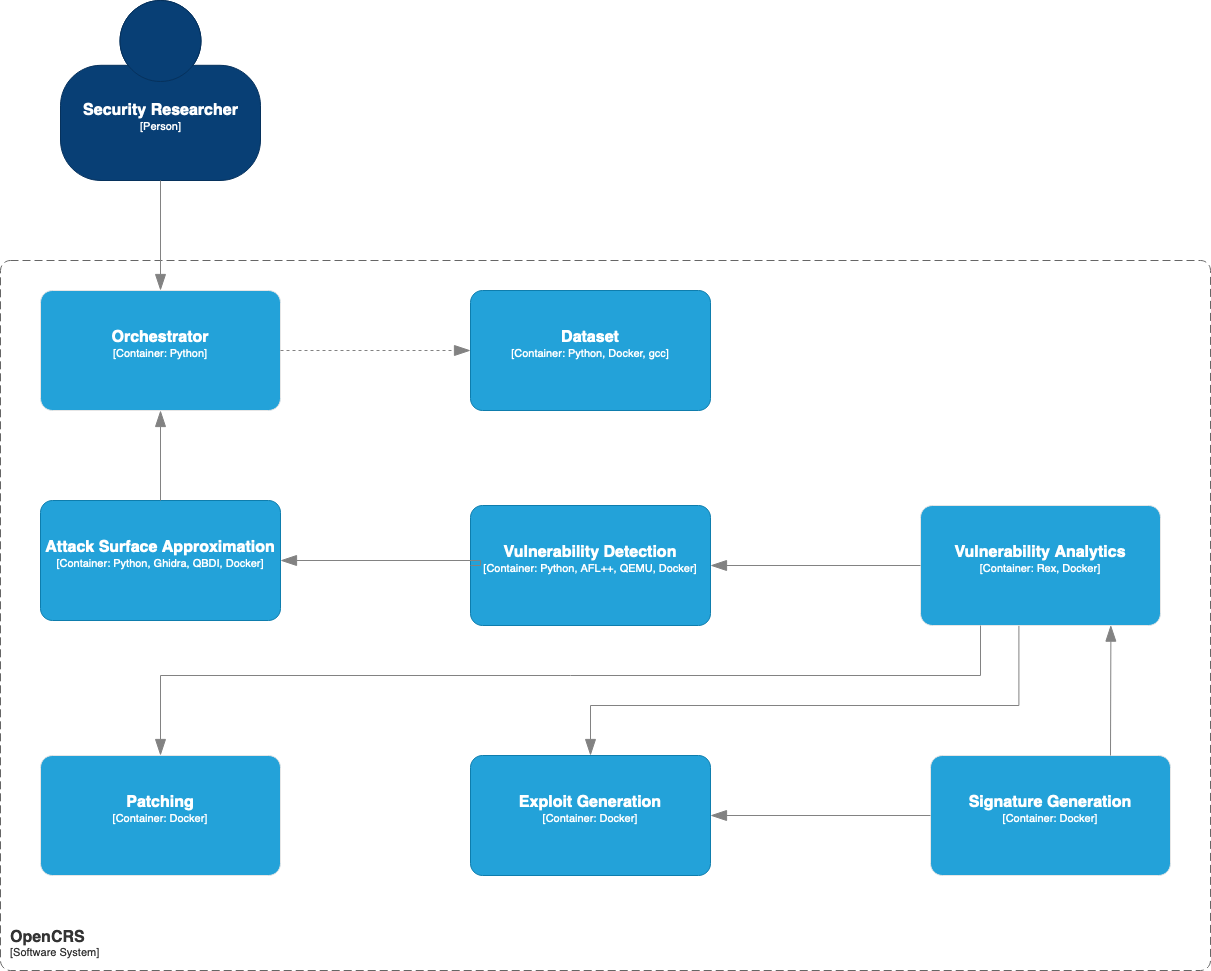
\includegraphics[width=0.8\textwidth, center]{images/opencrs.png}
	\captionsetup{justification=centering,margin=1cm}
	\captionof{figure}{OpenCRS's Architecture}
\end{frame}

\begin{frame}
	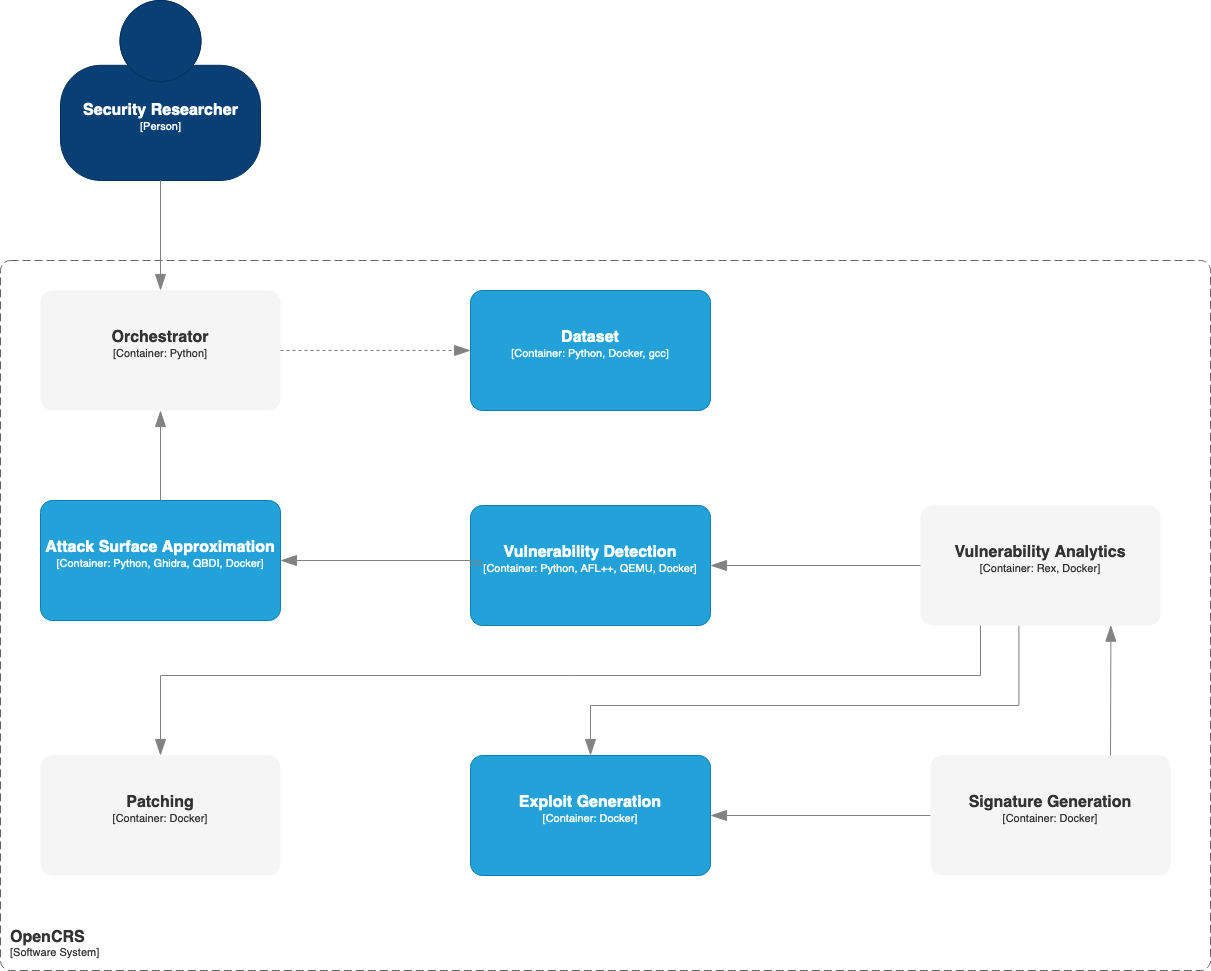
\includegraphics[width=0.8\textwidth, center]{images/highlighted.png}
	\captionsetup{justification=centering,margin=1cm}
	\captionof{figure}{OpenCRS Modules To Be Discussed}
\end{frame}